\subsection{Interrelación Asignatura Curso Académico - Calificación Alumno
            Asignatura CA}

   \begin{description}
      \item[Definición] En esta interrelación se deja constancia de que un
      alumno obtendrá una calificación de una asignatura en una determinada
      convocatoria durante un curso académico.

      \begin{itemize}
       \item Una \textit{Asignatura Curso Académico} puede tener varias
             \textit{Calificación Alumno Asignatura CA}.
       \item Una \textit{Calificación Alumno Asignatura CA} solamente puede
             pertenecer a una \textit{Asignatura Curso Académico}.
      \end{itemize}

      \item[Características] La interrelación presenta las siguientes
                             características:

         \begin{itemize}
            \item \textbf{Nombre:} ACA-Cal
            \item \textbf{Tipo de la interrelación:} El tipo de entidad
                  Calificación Alumno Asignatura CAes débil por identificación
                  respecto al tipo de entidad Alumno Curso Académico.
            \item \textbf{Cardinalidad de la interrelación:} 1:N
                  \begin{itemize}
                     \item Asignatura Curso Académico: tiene (0,n)
                     \item Calificación Alumno Asignatura CA: pertenece\_a (1,1)
                  \end{itemize}
            \item \textbf{Número de atributos:} Ninguno.
         \end{itemize}

      \item[Diagrama] La figura \ref{diagramaACA-Cal} muestra el diagrama de la
                      interrelación.

      \item \begin{figure}[!ht]
            \begin{center}
            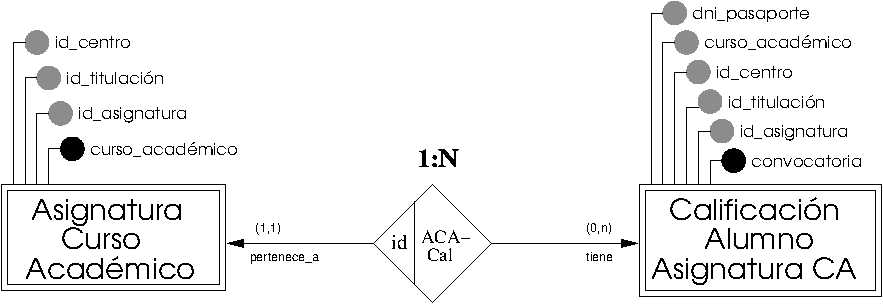
\includegraphics[]{07.Modelo_Entidad-Interrelacion/7.3.Analisis_Interrelaciones/diagramas/ACA-Cal.pdf}
            \caption{Diagrama de la interrelación ACA-Cal.}
            \label{diagramaACA-Cal}
            \end{center}
         \end{figure}

      \item[Ejemplo práctico del tipo de interrelación]

      \item \begin{center}
            \begin{tabular}{ | r r | }
            \hline
            \multicolumn{2}{ | c | }{\textbf{Tipo de interrelación ACA-Cal}} \\
            \hline
            \textbf{Asignatura Curso Académico} & \\
            id\_centro & 15 \\
            id\_titulación & 3\\
            id\_asignatura & 17\\
            curso\_académico & 2008\\
            \hline
            \textbf{Calificación Alumno Asignatura CA} & \\
            dni\_pasaporte & 01234567A \\
            curso\_académico & 2008 \\
            id\_centro & 15 \\
            id\_titulación & 3\\
            id\_asignatura & 17\\
            convocatoria & febrero \\
            \hline
            \end{tabular}
         \end{center}
   \end{description}
